\documentclass[11pt]{article}
\usepackage{fullpage,amsthm,amsfonts,amssymb,epsfig,amsmath}

\begin{document}

\begin{center}
{\bf\large HW4 - S15}\\
Handed out 4-21 \hfill Warmuth/Rahmanian \hfill 4-28, beg. of class \\
\end{center}

\begin{enumerate}
\item$\;$

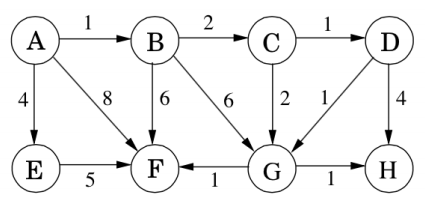
\includegraphics[width=7in]{DPV41.PNG}
\item$\;$

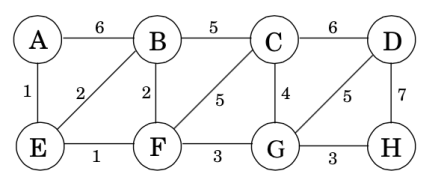
\includegraphics[width=7in]{DPV51.PNG}
\item
Often there are multiple shortest paths between two nodes
of a graph. How do you need to modify Dijkstra's algorithm
so that it finds the number of shortest paths.
\item
Recall that the correctness proof of Dijkstra's algorithm
assumes that the weights of the edges are non-negative.
Give a small example digraph with some negative edges
where Dijkstra's algorithm does not find the shortest path.
\newpage
\item$\;$

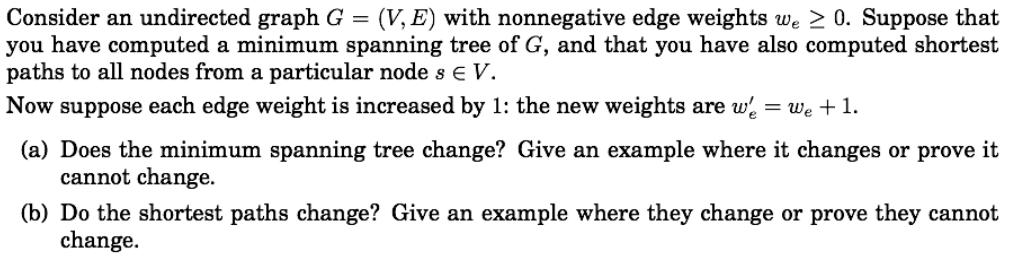
\includegraphics[width=7in]{DPV55.PNG}
\item
KT, Problem 2, p. 189
%\item
%KT, Problem 24, p. 200
%\item
%Argue that the solution to the recurrence
%$T(n)=T(n/3)+T(2n/3)+cn$, where $c$ is a positive constant
%is $\Omega(n \log n)$ by appealing to the recursion tree.
\end{enumerate}
\end{document}
